\documentclass[12pt]{article}
\usepackage{fullpage,amsmath,amsfonts,mathpazo,microtype,nicefrac, graphicx}

% Set-up for hypertext references
\usepackage{hyperref,color,textcomp,listings}

\definecolor{RoyalBlue}{rgb}{0,0,0.9}
\hypersetup{
   colorlinks=true,
   hypertexnames=true, pdfhighlight=/O,
   urlcolor=RoyalBlue, linkcolor=RoyalBlue}

\hypersetup{pdftitle={User Manual}}

% Macro definitions
\newcommand{\N}{\mathbb{N}}
\newcommand{\Z}{\mathbb{Z}}
\newcommand{\Q}{\mathbb{Q}}
\newcommand{\R}{\mathbb{R}}
\newcommand{\p}{\partial}
\renewcommand{\vec}[1]{\mathbf{#1}}
\newcommand{\vx}{\vec{x}}
\newcommand{\vp}{\vec{p}}
\newcommand{\Trans}{\mathsf{T}}

\begin{document}
\title{The \textsc{pychemkin} User Manual}
\author{Jane Huang, Kimia Mavon, Weidong Xu, Zeyu Zhao}
\date{}
\maketitle
\section{Introduction}


{\tt pychemkin} is a Python 3 library that computes the reaction rates of species participating in a system of elementary reactions.

\subsection{Key chemical concepts and terminology}

A system consisting of $M$ elementary reactions involving $N$ species has the general form
\begin{align}
  \sum_{i=1}^{N}{\nu_{ij}^{\prime}\mathcal{S}_{i}} \longrightarrow
  \sum_{i=1}^{N}{\nu_{ij}^{\prime\prime}\mathcal{S}_{i}}, \qquad j = 1, \ldots, M.
\end{align}
for \textbf{irreversible reactions} (i.e., the reaction only proceeds in the forward direction) and 

\begin{align}
  \sum_{i=1}^{N}{\nu_{ij}^{\prime}\mathcal{S}_{i}} \rightleftharpoons
  \sum_{i=1}^{N}{\nu_{ij}^{\prime\prime}\mathcal{S}_{i}}, \qquad j = 1, \ldots, M.
\end{align}
for \textbf{reversible reactions} (i.e., the reaction can proceed in either the forward or backward directions). 

$S_i$ is the $i$th specie in the system, $\nu_{ij}^{\prime}$ is its stoichiometric coefficient (dimensionless) on the reactants side of the $j$th reaction, and $\nu_{ij}^{\prime\prime}$ is its stoichiometric coefficient (dimensionless) on the product side for the $j$th reaction.

Each specie is characterized by a concentration $x_i$, in units of [mol/vol].
The \textbf{reaction rate} of each specie is the time rate of change of its concentration, $\frac{dx_i}{dt}$. The reaction rate is usually represented by the symbol $f_i$, such that
\begin{align}
  f_{i} = \sum_{j=1}^{M}{(\nu_{ij}^{\prime\prime}-\nu_{ij}^\prime)\omega_{j}}= \sum_{j=1}^{M}{\nu_{ij}\omega_{j}}, \qquad i = 1, \ldots, N.
\end{align}

The \textbf{progress rate} of the $j$th reaction is given by


\begin{align}
\omega_{j} = k_{j}^{\left(f\right)}\prod_{i=1}^{N}{x_{i}^{\nu_{ij}^{\prime}}} - k_{j}^{\left(b\right)}\prod_{i=1}^{N}{x_{i}^{\nu_{ij}^{\prime\prime}}}, \qquad j = 1,\ldots, M.
\end{align}

The \textbf{forward reaction rate coefficient} $k_j^{\left(f\right)}$ is assumed to take one of three possible forms:
\begin{enumerate}
\item $k=$ constant
\item Arrhenius: $k=A\exp(-\frac{E}{RT})$, where $A$ is the pre-factor, $E$ is the activation energy, $R$ is the universal gas constant, and $T$ is the temperature.
\item Modified Arrhenius: $k=AT^b\exp(-\frac{E}{RT})$, where $A$ is the pre-factor, $E$ is the activation energy, $R$ is the universal gas constant, $T$ is the temperature, and $b$ is the temperature scaling parameter.
\end{enumerate}

The forward and backward reaction rate coefficients are related by 
\begin{align}
k_{j}^{\left(b\right)} = \frac{k_{j}^{\left(f\right)}}{k_{j}^{e}}, \qquad j =1, \ldots, M,
\end{align}
where the \textbf{equilibrium coefficient} $k_{j}^{e}$ is given by 
\begin{align}
k_{j}^{e} = \left(\frac{p_{0}}{RT}\right)^{\gamma_{j}}\exp\left(\frac{\Delta S_{j}}{R} - \frac{\Delta H_{j}}{RT}\right), \qquad j =1, \ldots, M.
\end{align}
The pressure $p_0$ is fixed at 10$^5$ Pa in this package. $\gamma_{j} = \sum_{i=1}^{N}{\nu_{ij}}$. The \textbf{entropy change} of reaction $j$ is  
\begin{align}
\Delta S_{j} = \sum_{i=1}^{N}{\nu_{ij}S_{i}}, \qquad j =1, \ldots, M,
\end{align}
where $S_i$ is the entropy of specie $i.$ Likewise, the \textbf{enthalpy change} of reaction $j$ is 
\begin{align}
\Delta H_{j} = \sum_{i=1}^{N}{\nu_{ij}H_{i}}, \qquad j =1, \ldots, M. 
\end{align}

An irreversible reaction can be thought of as the limiting case where $k_{j}^{e}$ approaches $\infty$, in which case the backwards reaction rate coefficient $k_{j}^{\left(b\right)}$ approaches 0. The progress rate expression then simplifies to 
\begin{align}
\omega_{j} = k_{j}^{\left(f\right)}\prod_{i=1}^{N}{x_{i}^{\nu_{ij}^{\prime}}}, \qquad j = 1,\ldots, M.
\end{align}
\subsection{Features}
The package can solve for the reaction rates of a system of elementary reactions. The number of reactions and species is arbitrary. For each system of reactions, the user supplies the species participating in the reactions, the chemical equations, the stoichiometric coefficients for the reactants and products, and the rate coefficient parameters (e.g., $E$ and $A$ for Arrhenius rates). For a given system, the user can then specify a temperature and a vector of species concentrations in order to return the reaction rates in the form of a NumPy array. Rate coefficients and reaction progress rates can also be retrieved. 

\subsubsection{Calculation of thermodynamic quantities}
Traditionally for combustion chemistry, the entropy and enthalpy of each species are approximated by polynomial fits to numerical calculations from Gordon and McBride's 1963 report, \textit{The Thermodynamic Properties of Chemical Substances to 6000 K, NASA Report SP-3001}:
\begin{equation}
\frac{H_{i}}{RT} = a_{i1} + \frac{1}{2}a_{i2}T + \frac{1}{3}a_{i3}T^{2} + \frac{1}{4}a_{i4}T^{3} + \frac{1}{5}a_{i5}T^{4} + \frac{a_{i6}}{T}
\end{equation}
and 
\begin{equation}
\frac{S_{i}}{R} = a_{i1}\ln\left(T\right) + a_{i2}T + \frac{1}{2}a_{i3}T^{2} + \frac{1}{3}a_{i4}T^{3} + \frac{1}{4}a_{i5}T^{4} + a_{i7}.
\end{equation}
These are known as the \textbf{NASA polynomials}. For each specie, there are two sets of coefficients $a_i$, the first of which is applicable at low temperatures and a second that is applicable at high temperatures. \texttt{pychemkin} stores these coefficients (taken from \url{http://burcat.technion.ac.il/dir/}) in an SQL database and retrieves values for species requested by the user (we have updated the SQL database which contains more species). 




\section{Installation}

\subsection{Where to find and download the code}
\subsubsection{Using pip}
\texttt{pychemkin} v. 0.1.1 is hosted on PyPi at \url{https://pypi.python.org/pypi/pychemkin}. To download and install the package, simply type 
\texttt{pip install pychemkin} into your terminal.
\subsubsection{Installing from source}

To get the most up-to-date version, you can go to \url{https://github.com/cs207group4/cs207-FinalProject}. If you have a GitHub account, you can simply open your terminal and type {\tt git clone git@github.com:cs207group4/cs207-FinalProject.git}. Otherwise, you can download the package by clicking on the green button in the upper right corner of the page that says "Clone or download," then click "Download ZIP" to download the entire repository as a ZIP file. Once you download the contents of the repository from GitHub, enter the directory and type {\tt python setup.py install} In order to run the test suite, you need to have \href{https://docs.pytest.org/en/latest/}{pytest} v. 3.00+ and \href{https://pypi.python.org/pypi/pytest-cov}{pytest-cov} v. 2.5+ installed. When you're in the top level of the package directory, type {\tt pytest} into the terminal. The results of the test code will be printed out to the terminal.
 \newline

\subsection{Dependencies}

This package has dependencies that usually come standard with the Anaconda distribution, but will otherwise automatically be installed for you if you use pip.
\begin{itemize}
\item \href{http://www.numpy.org/}{NumPy} v. 1.11+
\item \href{https://www.sqlite.org/}{sqlite3} v. 3.13.0+
\item \href{https://www.scipy.org/}{SciPy} v. 1.0.0+
\end{itemize}

\section{Basic Usage and Examples}
As an example of basic code usage, we consider the following system of elementary, irreversible reactions:

\begin{enumerate}
\item H + O$_2$ $\overset{k_1}{\rightarrow}$ OH + O
\item H$_2$ + O $\overset{k_2}{\rightarrow}$OH + H
\item H$_2$ + OH $\overset{k_3}{\rightarrow}$ H$_2$O + H
\end{enumerate}

Reaction 1 has an Arrhenius rate coefficient with $A = 3.52\times 10^{10}$ and $E = 7.14\times 10^4$. Reaction 2 has a modified Arrhenius rate coefficient with $A = 5.06\times 10^{-2}$, $b = 2.7$, and $E = 2.63\times10^4$. Finally, reaction 3 has a constant rate coefficient of $k_3 = 10^3$.



\subsection{User-required input}
In an xml input file, the user provides the species participating in the reactions, the chemical equations, the stoichiometric coefficients, and the rate coefficient parameters. See {\tt rxns.xml} in the {\tt tests/test\_xml} folder for an example of how to format the input file. 

The xml file will be processed and stored in a {\tt chemkin} object as follows:
\begin{lstlisting}[language = Python, basicstyle = \ttfamily, breaklines = True, columns = fullflexible]
>>>from pychemkin import chemkin
>>>rxn_system = chemkin.from_xml('rxns.xml')
Finished reading xml input file
\end{lstlisting}

We can print out information about the reaction system as follows:
\begin{lstlisting}[language = Python, basicstyle = \ttfamily,columns = fullflexible, showstringspaces = False]
>>>print(rxn_system)
chemical equations:
[
H + O2 =] OH + O
H2 + O =] OH + H
H2 + OH =] H2O + H
]
species: [`H', `O', `OH', `H2', `H2O', `O2']
nu_react:
[[ 1.  0.  0.]
 [ 0.  1.  0.]
 [ 0.  0.  1.]
 [ 0.  1.  1.]
 [ 0.  0.  0.]
 [ 1.  0.  0.]]
nu_prod:
[[ 0.  1.  1.]
 [ 1.  0.  0.]
 [ 1.  1.  0.]
 [ 0.  0.  0.]
 [ 0.  0.  1.]
 [ 0.  0.  0.]]
reaction coefficients:
[
Arrhenius Reaction Coeffs: {`A': 35200000000.0, `E': 71400.0, `R': 8.314}
modifiedArrhenius Reaction Coeffs: {`A': 0.0506, `b': 2.7, `E': 26300.0, `R': 8.314}
Constant Reaction Coeffs: {`k': 1000.0, `R': 8.314}
]
reaction types: [`Elementary', `Elementary', `Elementary']
reversible: [`no', `no', `no']
\end{lstlisting}


\subsection{Computing reaction rates}
Given the reaction data from a user-provided input file, the reaction rates can be computed for an arbitrary temperature and set of species concentrations.

\begin{lstlisting}[language = Python, basicstyle = \ttfamily,columns = fullflexible, showstringspaces = False]
>>> T = 1000 #K
>>> x = np.array([1,1,1,1,1,1])
>>> rxn_system.reaction_rate_T(x,T)
array([ -6.28889929e+06,   6.28989929e+06,   6.82761528e+06,
            -2.70357993e+05,   1.00000000e+03,  -6.55925729e+06])
\end{lstlisting}

\subsection{Obtaining intermediate calculations}
Rate coefficients and progress rates are calculated in the course of computing the reaction rates. While these methods do not have to be called by the user to obtain the reaction rates, they are accessible if the user wishes to obtain these values. 

\subsubsection{Obtaining forward rate coefficients}
While the xml file provides the parameters for the functional form of the rate coefficient expression, a temperature (usually) has to be specified to compute the rate coefficient. Our package does this in the following manner:

\begin{lstlisting}[language = Python, basicstyle = \ttfamily,columns = fullflexible, showstringspaces = False]
>>> from pychemkin import ReactionCoeffs
>>> rc = ReactionCoeffs(`Arrhenius', A = 1e7, E=1e3)
>>> rc.set_params(T=1e2)
>>> rc.k_forward()
    3003549.0889639612
\end{lstlisting}


\subsubsection{Obtaining progress rates}
The progress rate values $w_i$ can be computed in the following manner:
\begin{lstlisting}[language = Python, basicstyle = \ttfamily,columns = fullflexible, showstringspaces = False]
>>> T = 1000 #K
>>>  x = np.array([1,1,1,1,1,1])
>>>  rxn_system.progress_rate(x,T)
array([  6.55925729e+06,   2.69357993e+05,   1.00000000e+03])
\end{lstlisting}

\subsection{Future features}
\subsubsection{Motivation}

We will design a package to allow for simulations of complex chemical processes (i.e., those that cannot be solved by hand/analytically) and to facilitate understanding of the key processes. Chemical kinetics simulations typically involve a series of coupled differential equations. Our package will solve these ODEs to obtain species concentrations as a function of time, and then visualize the results to enable the user to identify key reactions and species at different times.

\subsubsection{How features will fit into the code base}

Currently, the package computes reaction rates for an arbitrary number of species and elementary reactions for a single time step. These ODEs will be input into an ODE solver to yield progress rates, reaction rates, and concentrations for multiple time steps. The solutions will be written to an output file (csv or HDF5), which can then be read by a visualization module. 

\subsubsection{Modules to realize the features}

\subsubsection*{Module 1: ChemSolver}


\texttt{ChemSolver} is a module built to wrap around \texttt{SciPy}'s ODE solver to obtain reaction concentrations. The user can choose one of the five algorithms available in \texttt{SciPy}, specify the time range over which to solve the ODEs, and select the output format (csv or HDF5). The user also has the option of exploring parameter space by running a grid of simulations with a single function call. 

The \texttt{scipy.integrate} library has a powerful routine, “\texttt{ode},” for numerically solving systems of coupled first order ordinary differential equations. \texttt{ChemSolver} allows the user to choose from the 5 algorithms incorporated in \texttt{scipy.integrate.ode}, depending on their needs and preferences. 
 
The user may specify the output of \texttt{ChemSolver} to be csv or HDF5.
\subsubsection*{Module2: ChemVis}

This module offers a visualization library for the output of ODE solver. It would read in the data from HDF5 or csv using \texttt{Pandas}. For the first type of visualization, users will be able to plot progress rates, reaction rates, or concentrations as a function of time. The user will be able to select a subset of species or a subset of the time range. For the second type of visualization, the relationship between species will be plotted in a social network style visual. This will provide the user an alternate view of major pathways and key species in the system. The output will be an image made with \texttt{Matplotlib}.  



\subsubsection{Methods to be implemented}
\texttt{Chemsolver} methods:

The differential equation we want to solve is
$$f = chemkin.reaction\_rate(X,T)$$
where X is the concentration vector and T is the temperature. 
The method we plan to write will be structured as:

\begin{lstlisting}[language = Python, basicstyle = \ttfamily, breaklines = True, columns = fullflexible]
>>> ChemSolver.solve(chemkin_object, X_initial,T, timesteps, odemethod = odemethod,  outputmethod = outputmethod, *args)
\end{lstlisting}

where \texttt{*args} are the extra arguments we have to pass through to \texttt{SciPy}.

\texttt{chemkin} is the \texttt{chemkin} object that will be used to compute reaction rates. 

\texttt{X} can either be a one-dimensional array of length $N$ (corresponding to $N$ species for a single reaction system) or a two-dimensional array of length $NxP$, where $P$ is the number of different starting concentration combinations that the user may wish to try. $T$ is either a float or a float array of length $P$, depending on whether the user wants to run multiple simulations. 

\texttt{timesteps} is an array specifying the points in time for which the user wishes for the concentrations to be output. 

The \texttt{odemethod} corresponds to one of the five \texttt{SciPy} ODE solver algorithms: 
This method will solve the ODE. The user will be able to chose from 5 ODE solvers: 
\begin{itemize}
\item ‘RK45’ (Explicit Runge-Kutta method of order 5(4))
\item ‘RK23’ (Explicit Runge-Kutta method of order 3(2))
\item ‘Radau’ (Implicit Runge-Kutta method of Radau IIA family of order 5.)
\item ‘BDF’ (Implicit method based on Backward Differentiation Formulas.)
\item ‘LSODA’ (Adams/BDF method with automatic stiffness detection and switching)
\end{itemize}

The output method allows the user to select either csv or HDF5 as an output option. The function will output a single file consisting of columns corresponding to time, reaction rates, species progress rates, species concentrations. There will also be a header storing the chemical equations. 


\subsubsection*{ChemVis Methods}

\begin{lstlisting}[language = Python, basicstyle = \ttfamily, breaklines = True, columns = fullflexible]
>>> ChemVis.plot_time_series(simulationfile, yaxis = yaxisval, species = [list of species], timerange = timerange)
\end{lstlisting}


This method will allow users to visualize species’ reaction rates or concentrations over time, or the reaction progress rates over time. 

\texttt{simulationfile} is a string or a list of strings corresponding the the csv or HDF5 file(s) containing the simulation data to be plotted (from \texttt{ChemSolver.solve}).

\texttt{yaxisval} is the quantity to be plotted: reaction rate or concentration

\texttt{species} is a list of species to be plotted.

\texttt{timerange} specifies the start and end time for the time series to be plotted (which can be a subset of the simulation run). 

A mock-up of the output image is shown below in Figure 1.



\begin{figure}[h!]
  \caption{This visual plots concentrations of two species over time. We can clearly see that while Species 1 starts off with a higher concentration, the concentration of Species 2 grows much faster than that of Species 1 (exponential growth). Users can alternatively choose reaction rates over time, or the reaction progress rates over time. }
  \centering
  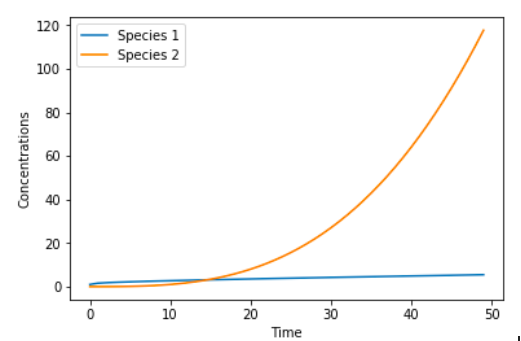
\includegraphics[width=0.6\textwidth]{pic1.png}
\end{figure}



\texttt{ChemVis.plot\_network} is an alternative method for visualizing the relationship between the species in the network. 

\begin{lstlisting}[language = Python, basicstyle = \ttfamily, breaklines = True, columns = fullflexible]
>>>ChemVis.plot_network(simulationfile,timepoint)
\end{lstlisting}
An example image is shown in Figure 2 of a 3-reaction system involving 6 species. Red lines indicate that the species directly react with one another. Single-headed arrows show which species are direct parents of other species. Double-headed arrows show which species interconvert. The sizes of the species bubbles can show relative concentration levels. 

\texttt{simulationfile} is the output csv or HDF5 file from \texttt{ChemSolver}. \texttt{timepoint} is the point in time for which the plot is being generated



\begin{figure}[h!]
  \caption{This visual shows a 3-reaction system involving 6 species. Red lines indicate that the species directly react with one another. Single-headed arrows show which species are direct parents of other species. Double-headed arrows show which species interconvert. In future analysis, the package will offer the sizes of the species bubbles in relation to the relative concentration levels. }
  \centering
  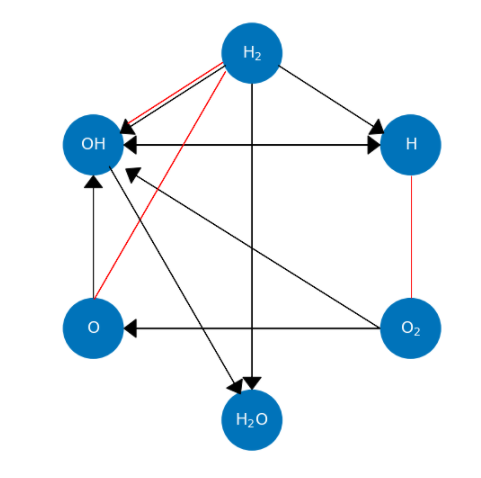
\includegraphics[width=\textwidth]{22.png}
\end{figure}

\newpage


\subsubsection{How to use the new feature}
Visualizing the species’ concentrations over time should allow the user to quickly identify these features of the chemical system:

\begin{itemize}

\item What are the roles of species in the system (primarily reactants, primarily intermediates, primarily products).
\item What bottlenecks are in the system?
\item What species are produced in high quantities and which ones consistently remain minor?

\end{itemize}

Additionally, visualizing progress rates and reaction rates over time will help the user understand what the major sources and sinks are for a given specie at a given time. 

The option of run and visualize a grid of models will allow the user to quickly explore parameter space and tune the starting concentrations and temperature to achieve desired production levels. For example, if the user wants to minimize the production of H2O2 for a given reaction system, she can provide a matrix of initial concentrations and quickly identify which starting concentration vector will yield the desired results. 

\subsubsection{External dependencies}
External dependencies include \texttt{SciPy, HDF5, Matplotlib}, and \texttt{Pandas}, in addition to \texttt{NumPy} and \texttt{sqlite3} mentioned in Section 2.2. 
\end{document}


